\section*{Appendix}

\noindent\textbf{Purchase100.} This dataset is a privacy sensitive dataset capturing the purchase preferences of online customers taken from the authors of~\cite{shokri2017membership}.
The data records have 600 binary features and each record is classified into one of 100 classes identifying each user's purchase.
For this dataset, we use a fully connected architecture with the nodes in each layers as [1024,512,256,128,100].

\noindent\textbf{Location.} This dataset is a privacy sensitive dataset capturing user's location "check-ins" taken from the authors of~\cite{shokri2017membership} where each record has 446 binary features which is mapped to one of 30 classes each representing a location. For this dataset we use a fully connected architecture with hyperparameters as [512,256,128,30].

\begin{figure}[!htb]
    \centering
    \begin{minipage}[b]{1\linewidth}
    \centering
    \subfigure[Pubmed]{
    \label{fig:mem_soft_label}
    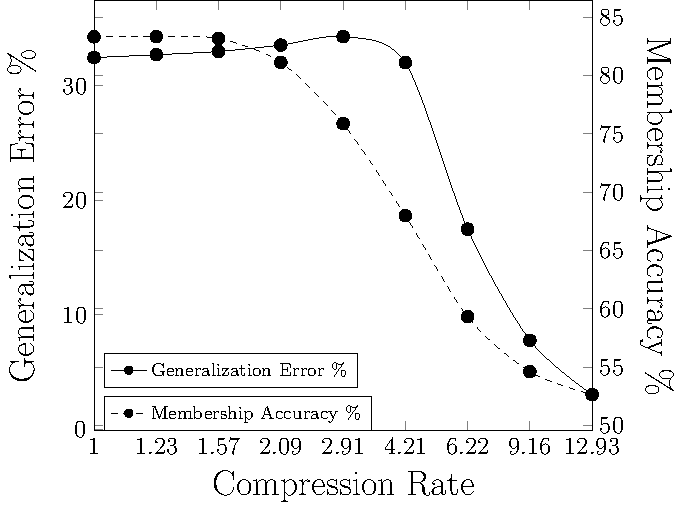
\includegraphics[width=0.5\linewidth]{figures/location_prune.pdf}
    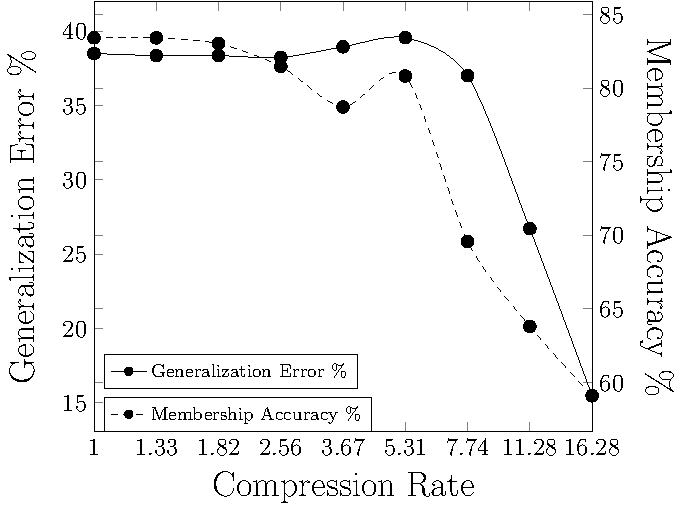
\includegraphics[width=0.5\linewidth]{figures/purchase_prune.pdf}
    }

    \subfigure[Citeseer]{
    \label{fig:nonmem_soft_label}
    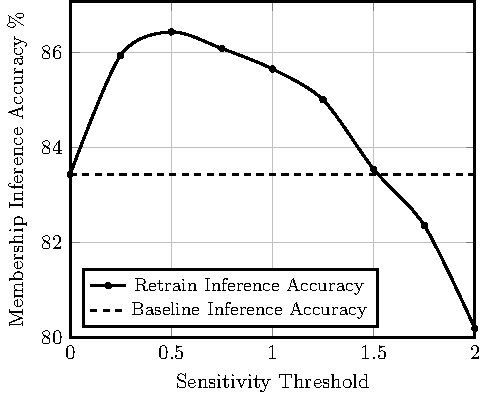
\includegraphics[width=0.5\linewidth]{figures/location_retrain.pdf}
    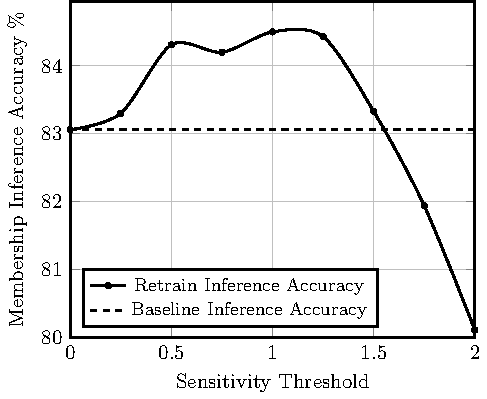
\includegraphics[width=0.5\linewidth]{figures/purchase_retrain.pdf}
    }

    \subfigure[Cora]{
   	\label{fig:mem_soft_label}
    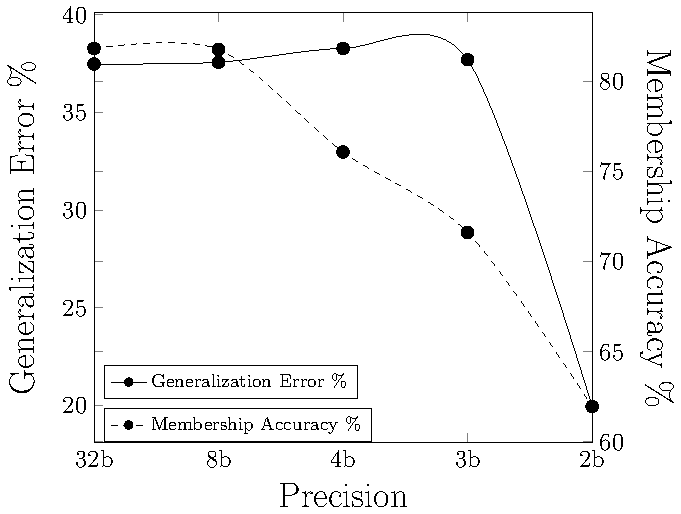
\includegraphics[width=0.5\linewidth]{figures/location_wtsharing.pdf}
    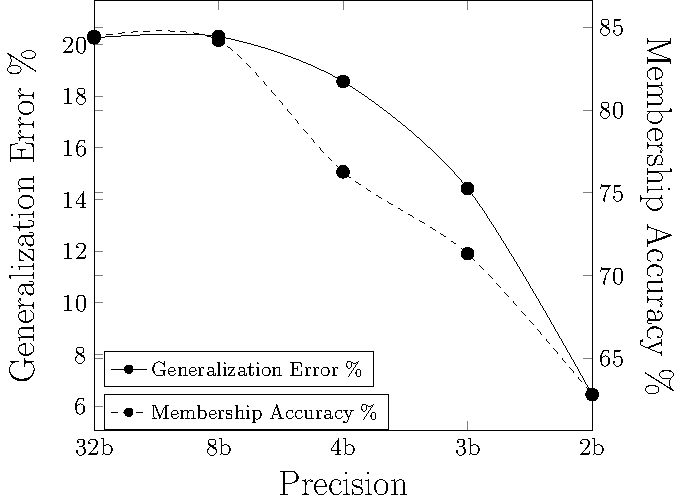
\includegraphics[width=0.5\linewidth]{figures/purchase_wtsharing.pdf}
    }

    \end{minipage}
    \caption{Model predictions are more confident for nodes in $G_{train}$ compared to test graph (left). The extent of overfitting can be detected by a non-overlapping region between the output prediction distributions across all data points (right).}
    \label{fig:NIAcause}
\end{figure}
